\chapter{Desarrollo del Proyecto}
\label{chap:desarrollo}

\drop{E}l presente capítulo describe todo el proceso de desarrollo del proyecto, incluidas aquellas fases que fueron meramente preparatorias e introductorias, así como la generación de cada uno de los prototipos.

Con el fin de conseguir la suficiente claridad en la exposición de los contenidos que se describen a continuación, las secciones en las que se divide el capítulo se corresponderán con las iteraciones descritas en el capítulo anterior (\hyperref[sec:fasesdetrabajo]{ver Sección~\ref{sec:fasesdetrabajo}}). 

\section{Iteración 0}

Como el lector seguramente ya habrá podido intuir, esta iteración es puramente de investigación, análisis y consideraciones de diseño, no obstante a continuación se detalla brevemente cómo y dónde han quedado abordados cada uno de los puntos expuestos en la \hyperref[sub:metodologiaiter0]{Subsección~\ref{sub:metodologiaiter0}}

\subsection{Requisitos}

Además de mi bagaje y experiencia en el sector de la seguridad durante más de 5 años en su totalidad, el apartado de requisitos se ha construido tras haber consultado la normativa de seguridad en España y haberme entrevistado con profesionales del sector de la seguridad cómo: Alejandro Moreno López (Técnico de Laboratorio y Puesta en Marcha, con más de 30 años de experiencia) y Antonio Salas Galiana (Gerente de Innovación y Calidad), ambos de la compañía \textit{Prosegur Soluciones S.A}\footnote{\url{https://www.prosegur.es/esp/legal/}}.

De este proceso introductorio, pero no por ello el menos importante, han salido los requisitos (funcionales y no funcionales). Con el fin de no resultar repetitivo, no se detallarán requisitos ya que estos se ven expuestos y quedan cubiertos en su totalidad en el \hyperref[chap:objetivos]{Capítulo~\ref{chap:objetivos} Objetivos}.

\subsection{Consideraciones de diseño}

Además de los aspectos que han sido expuestos en los puntos que se describen en la \hyperref[sub:metodologiaiter0]{Subsección~\ref{sub:metodologiaiter0}} y que se han abordado en los Capítulos \hyperref[chap:objetivos]{\ref{chap:objetivos}} y \hyperref[chap:antecedentes]{\ref{chap:antecedentes}}, también existen otros que son importantes para la elección del marco de desarrollo de este proyecto:

\begin{itemize}
  \item Uno de los requisitos es conseguir una capacidad de integración que permita la gestión de diferentes elementos y subsistemas de seguridad, propios o de terceros.
  \item En un primer momento no tenía claro qué \textit{framework} y lenguaje de programación emplear para el desarrollo de lo que sería la aplicación web del sistema.
  \item Mi mayor experiencia en el desarrollo de aplicaciones la tenía con el lenguaje \textit{Ruby}\footnote{\url{https://www.ruby-lang.org/es/}} y el \textit{framework} \textit{Rails}\footnote{\url{http://www.rubyonrails.org.es/}}, que a pesar de contar con una amplia comunidad y soporte, desgraciadamente no era completamente multiplataforma y tampoco compatible con la parte servidor  del sistema de emulación hardware que más tarde desarrollaría con \textit{Zero C-Ice}\footnote{\url{https://zeroc.com/}}.

\end{itemize}

Tomando las cuestiones anteriores en cuenta, llegué a la conclusión de que necesitaba un lenguaje multiplataforma con el que estuviese familiarizado, con una curva de aprendizaje rápida y una amplia comunidad de desarrolladores, donde pudiese encontrar ejemplos, documentación y un buen soporte en su uso. El otro lenguaje que conocía que reuniese todas estas características, además de \textit{Ruby} era \textit{Python} y por fortuna existía un marco de desarrollo web basado en él, \textit{Django}\footnote{\url{https://www.djangoproject.com/}}.

\section{Iteración 1}

Esta iteración cubre todos los aspectos descritos en la \hyperref[sub:metodologiaiter1]{Sección~\ref{sub:metodologiaiter1}} y además aporta familiaridad y conocimientos de los entornos de desarrollo, Arduino y AngularJS, que más tarde se emplearán para el desarrollo evolutivo del prototipo.

\subsection{Ejemplo: «Sistema básico de Seguridad»}

Este ejemplo trata de ilustrar y comprobar la fidelidad de las mediciones de la placa \hyperref[tab:arduino-yun]{\textit{Arduino-Yún}} o cualquier otra de la familia Arduino, mediante la realización de un ejercicio teórico que simula el comportamiento real ante una intrusión en una sucursal bancaria. He de aclarar que el ejemplo, \textit{BasicAlarmSystem}\footnote{\url{http://fritzing.org/projects/basicalarmsystem}} es libre y gratuito y su \href{https://github.com/AlejandroFerroBejerano/testAlarmaB-sico/blob/master/testAlarmaBasico.ino}{\textbf{código fuente}} está a \textbf{disposición de la comunidad}\footnote{\url{https://github.com/AlejandroFerroBejerano/testAlarmaB-sico}}. 

\subsubsection{Descripción del entorno}

Todos los datos proporcionados o cualquier similitud de la operativa aplicada con cualquier otra del mundo real es mera casualidad.

La sucursal 2741 de la entidad bancaria Santander, cuenta al igual que sus homólogos en el resto del territorio nacional, con varias mesas y mostradores que conforman los puestos de trabajos de sus empleados, así como con una caja fuerte donde se guarda todo el efectivo de la entidad. Para proteger todos los bienes materiales y humanos, la entidad cuenta con pulsadores de atraco silenciosos que avisan a la \acs{CRA} y un contacto magnético de tipo lapa en la puerta de la caja fuerte.

\subsubsection{Comportamiento del sistema}

A continuación se expone paso a paso cómo se ha concebido el ejemplo y las conclusiones al final de su ejecución. 

\begin{definitionlist}
\item[Comandos del sistema:] Son los comandos introducidos a través de la consola abierta por puerto serie con la placa.

\begin{itemize}
\item \textbf{Armar sistema:} Tecla «A» + tecla Entrar\footnote{\url{https://en.wikipedia.org/wiki/Enter_key}}.
\item \textbf{Desarmar sistema:} Tecla «D» + tecla Entrar.
\item \textbf{Silenciar sistema:} Tecla «S» + tecla Entrar.
\item \textbf{Rearmar sistema:} Tecla «R» + tecla Entrar.
\end{itemize}

\item[Sistema desarmado:] Cuando el sistema esté desarmado solo seguirán en funcionamiento los pulsadores de atraco y la comunicación con la \acs{CRA} mediante el visor de eventos. 

\item[Sistema armado:] Si el sistema se arma cualquier evento anormal (tamper o cortocircuito) en las zonas supervisadas generará una alarma. Además, el sistema sigue manteniendo activas las comunicaciones y los pulsadores. Al producirse una alarma por alguna de las zonas supervisadas (A0 -A5) como puede ser el magnético de la caja fuerte se activarán tanto la sirena lumínica como sonora y un relé que enciende todas las luces de la entidad. Si se activase una alarma silenciosa (pulsadores de atraco o pánico) solo se encienden las sirenas o indicadores luminosos.

\item[Guión de validación del ejemplo:] A las 8:00 abre la sucursal y el director de la misma accede a su despacho y comienza con sus labores rutinarias de trabajo. A las 11:30 entra un ladrón al banco y amenaza al director de la entidad con un arma. Pide que se le entregue el dinero de la caja fuerte y uno de los empleados presiona el botón de pánico sucediendo lo siguiente:

\begin{enumerate}
\item 11:31 - El vigilante de la \acs{CRA} visualiza la alarma silenciosa de atraco, silencia el aviso en pantalla y notifica inmediatamente a las fuerzas del orden.
\item 11:33 - Las sirenas de la policía alertan al ladrón de la inminente llegada y este sale corriendo despavorido sin un solo centavo de la sucursal.
\item 14:30 - Se cierra la oficina para contar el dinero.
\item 14:31 - El director de la entidad llama a la CRA para que desactiven la alarma y proceder al recuento. Se desactiva la alarma.
\item 14:40 - Se llama a la CRA para que se arme el sistema y todos se marchan.
\item 22:50 - El ladrón regresa a la oficina, hace un agujero en el cristal y accede a la habitación de la caja fuerte.
\item 23:15 - El ladrón corta las bisagras de la caja y manipula los cables del magnético para cortocircuitarlos y simular un estado normal. En ese mismo instante y de manera simultánea:
\begin{enumerate}
\item Salta la alarma, sonando la sirena y se encienden todas las luces de la entidad.
\item El vigilante de la CRA visualiza la alarma y avisa a la policía.
\end{enumerate}
\item 23:16 - El ladrón sale huyendo y es capturado unas calles más adelante.
\item 23:18 - Se rearma el sistema y se precinta la entidad.
\end{enumerate}

\item[Conclusiones:] Después de montar el circuito necesario para la ejecución del ejemplo (ver Figura~\ref{fig:sketchfritzing}) y seguir el guión establecido, he podido comprobar que cualquier placa de la familia Arduino podría ser capaz de supervisar un escenario igual o un poco más complejo del descrito. 

\end{definitionlist}

\begin{figure}[!h]
\centering
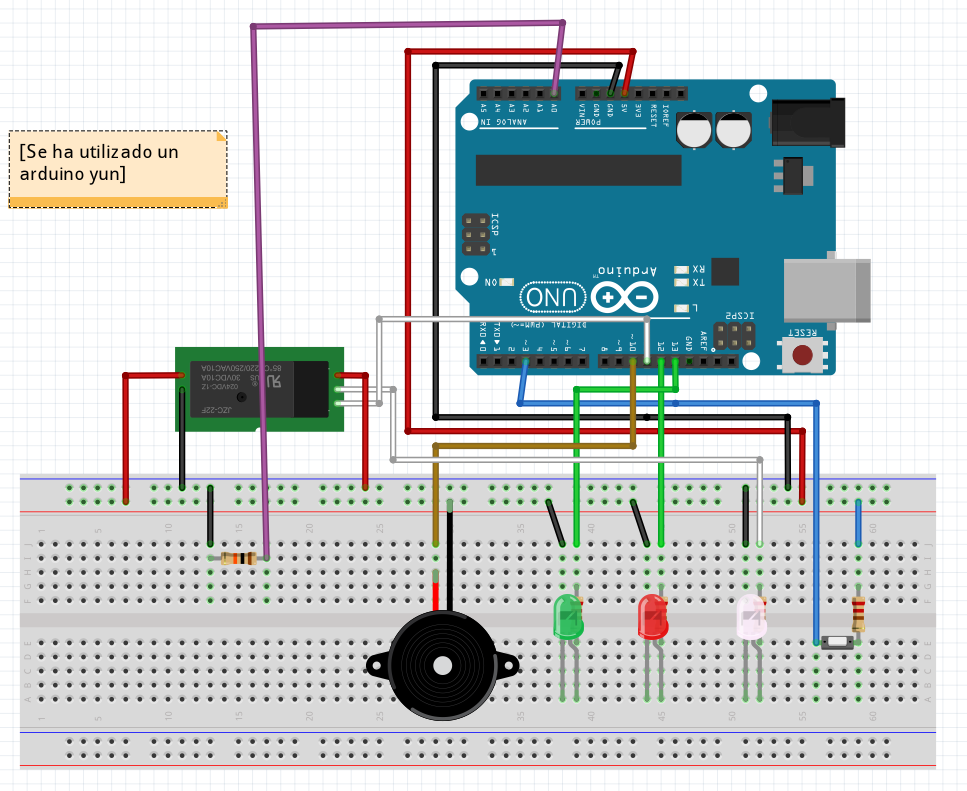
\includegraphics[width=0.7\textwidth]{/sketchfritzing.png}
\caption{Circuito necesario para la ejecución del ejemplo: «Sistema básico de Seguridad»}
\label{fig:sketchfritzing}
\end{figure}

\subsection{Ejemplo: «Yun-Webpanel»}

Tras haber usado el ejemplo anterior como base para probar las capacidades de las placas Arduino, en un entorno de seguridad, tocaba indagar en las nuevas capacidades que ofrece, en exclusiva la placa \hyperref[tab:arduino-yun]{\textit{Arduino-Yún}}. Como en el ejemplo anterior se explotaron las capacidades de lectura de los sensores (entradas analógicas A0-A5), en este se ha decidido probar el funcionamiento de las salidas en placa y su gestión desde una interfaz web (ver Figura~\ref{fig:yunwebpanel}). Para ello y al igual que venimos haciendo se ha elegido una historia o contexto práctico sobre la que aplicar el ejemplo.

He de especificar que el ejemplo, \textit{Yun-WebPanel}\footnote{\url{https://github.com/AlejandroFerroBejerano/Yun-Webpanel/blob/master/LICENSE}} es libre y gratuito y su \href{https://github.com/AlejandroFerroBejerano/Yun-Webpanel}{\textbf{código fuente}} está a \textbf{disposición de la comunidad}\footnote{\url{https://github.com/AlejandroFerroBejerano/Yun-Webpanel}}. 

\begin{figure}[h]
\centering
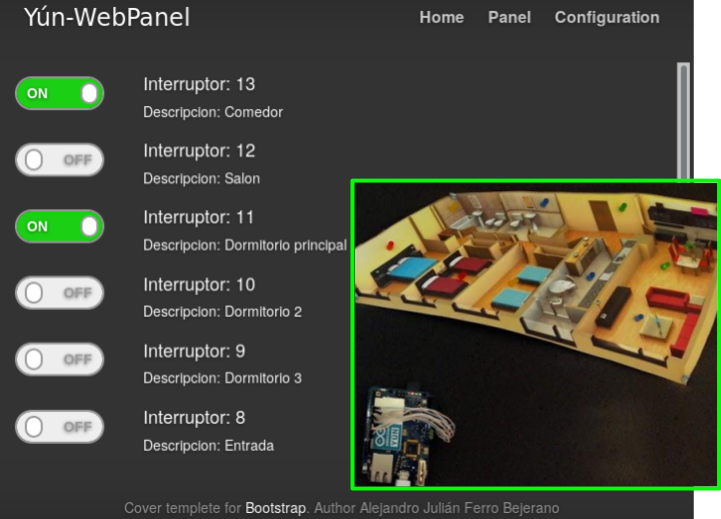
\includegraphics[width=0.8\textwidth]{/yun_webpanel.png}
\caption{Panel de ejemplo: «Yun-WebPanel»}
\label{fig:yunwebpanel}
\end{figure}


\begin{definitionlist}
\item[«Yun-WebPanel»] Es un panel web que permite el control domótico de viviendas o recintos, permitiendo al usuario la interacción con los elementos del mismo, ya sea local  o remotamente a través de un navegador web. 

\item[Librería explotada:] Este ejemplo muestra como explotar la biblioteca \textit{Bridge}\footnote{\url{https://www.arduino.cc/en/tutorial/bridge}} para modificar el estado de las salidas de la placa, en nuestro caso práctico encender y apagar las luces de una vivienda. Para facilitar la ejecución de nuestro ejemplo se ha dejado la contraseña \acs{REST}\footnote{\url{https://en.wikipedia.org/wiki/Representational_state_transfer}} deshabilitada, pudiéndose usar una  estructura \textit{url} o \textit{endpoints}\footnote{\url{https://github.com/Mach-II/Mach-II-Framework/wiki/Introduction-to-REST-Endpoints}} específico (ver Listado~\ref{code:yun_rest}).

\hfill
\lstinputlisting[label = {code:yun_rest}, caption = {Uso de la interfaz REST en Arduino-Yún~\cite{Bridge}}, style=customhttp]{code/yun_rest_endpoint.http}

\item[Requisitos:] Tener el equipo desde el que se interactúa en la misma red o enrutado con la interfaz ethernet de la placa \hyperref[tab:arduino-yun]{\textit{Arduino-Yún}}.

\item[Conclusiones:] Tras haber concluido con la construcción del ejemplo (código y maqueta), he podido comprobar de primera mano el potencial que ofrece la placa \hyperref[tab:arduino-yun]{\textit{Arduino-Yún}} para la gestión de salidas. Si extrapolamos esto al sector de la seguridad, estaríamos hablando de la interacción automática con toda clase de elementos que se puedan activar a través de un relé\footnote{\url{https://en.wikipedia.org/wiki/Relay}} como por ejemplo: sirenas, cerraderos, focos sorpresivos, barreras de vehículos, ventosas, luminosos, etc.

\end{definitionlist}

\section{Iteración 2}

Habiendo comprobado de primera mano las capacidades que nos ofrece la plataforma Arduino, comprendemos que la elaboración de todo el sistema para la publicación de eventos en nuestra aplicación web puede llegar a ser costosa en tiempos. Por ello y con el fin de poder agilizar las fases de desarrollo y las pruebas de concepto y software, en esta iteración me he centrado en la elaboración de un método que emule el comportamiento de las controladoras hardware del sistema (plataforma Arduino) y que facilite la generación de los estados físicos típicos de un sistema \acs{GIII} a través de plantillas predefinidas.

\subsection{Sistema de emulación}

Para nuestro sistema de emulación de las controladoras hardware se ha empleado un sistema distribuido muy sencillo, utilizando Zero C-Ice, donde se pueden identificar claramente dos partes (ver Figura~\ref{fig:1_classes_collector})

\begin{itemize}
  \item[Cliente:] Es el que lee la plantilla con los estados físicos definidos, para simular el comportamiento de los detectores y salidas conectados a la controladora hardware. Envía estos datos en bruto al servidor.
  \item[Servidor:] Tiene la función de recolectar la información, procesarla, darle un formato legible e imprimirla por pantalla para poder hacer un seguimiento visual de los eventos que se van produciendo. En posteriores iteraciones este recolector tendrá otras funciones más avanzadas.
\end{itemize}

\begin{figure}[h]
\centering
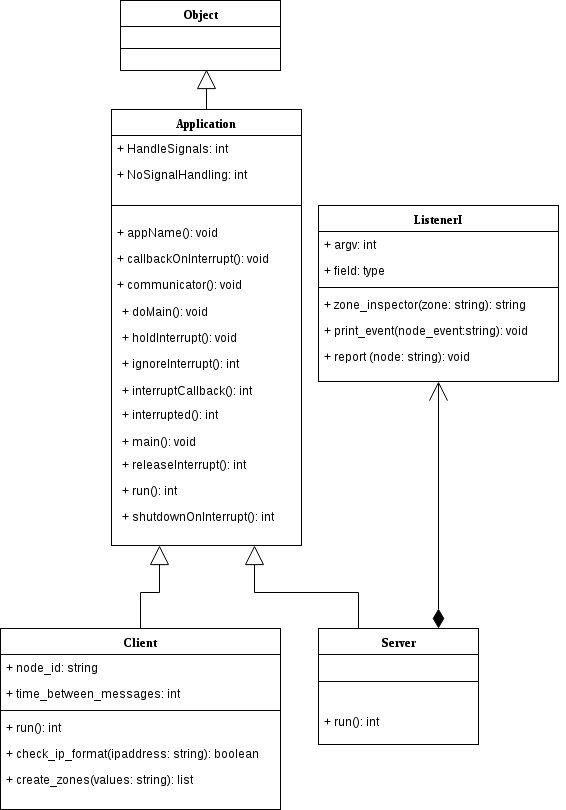
\includegraphics[width=0.8\textwidth]{/1_classes_collector.png}
\caption{Diagrama de clases del entorno de emulación}
\label{fig:1_classes_collector}
\end{figure}

Veamos a continuación algunos de los métodos más importantes.

\textbf{Métodos del cliente:}

\begin{itemize}
  \item \textbf{+ run( ):int} Método principal desde el cual comienza la ejecución del código cliente. Desde él se llaman al resto de métodos que abordan una funcionalidad específica y que pueden ser reutilizados si así se requiere. Si la ejecución es satisfactoria devuelve un 0, en caso contrario se lanza una excepción.
  \item \textbf{+ check\_ip\_format(ipaddress: string):boolean} Comprueba si en la dirección que se le proporciona al cliente, existe un socket escuchando al que pueda enviar la información. 
  \item \textbf{+ create\_zones(values: string): list} Procesa la cadena leída de la plantilla de emulación de estados y retorna una lista con un esquema muy sencillo que contiene el valor del detector o zona, asociado a su controladora (ver Listado~\ref{retval:client.create_zones}).
\end{itemize}

\lstinputlisting[label = {retval:client.create_zones}, caption = {Valor de retorno del método \textbf{+ create\_zones(values: string): string} }, style = customconsole]{code/client.create_zones.retval}

\textbf{Métodos del servidor:}

\begin{itemize}
  \item \textbf{+ run( ):int} Método principal desde el cual comienza la ejecución del código relativo a las comunicaciones del servidor. Si la ejecución es satisfactoria devuelve un 0, en caso contrario lanza una excepción.
  \item \textbf{+ zone\_inspector(zone: string):string} Evalúa, según el valor de tensión que se está reportando, el estado físico en que se encuentra el detector y el retorna un diccionario con la información básica acerca del valor leído del detector (ver Listado~\ref{retval:server.zone_inspector}). Los valores tomados como referencia para los umbrales fueron establecidos tras hacer mediciones forzando cada uno de los estados descritos (ver Cuadro~\ref{tab:zone_inspector_thresholds}) y teniendo en cuenta un cableado de 0,22 mm de diámetro (estándar para cableado de detectores y sensores en entornos de seguridad) y una distancia entre 0m y 100m. 

  \item \textbf{+ print\_event(node\_event: string): void} Como seguramente el lector puede asociar, este método se dedica exclusivamente a la impresión por pantalla de los eventos que se van sucediendo en un formato sencillo y fácil de seguir (ver Listado~\ref{retval:server.print_event}). Entiéndase por eventos a los sucesivos cambios de estados que se reportan desde los detectores o zonas.
  \item \textbf{+ report(node: string): void} Es el método que utilizan los clientes para que el servidor procese y trate toda la información que se le facilite. Desde este método se llaman a los métodos auxiliares que aportan una funcionalidad específica y que pueden ser reutilizados si así se requiere.
\end{itemize}

\lstinputlisting[label = {retval:server.zone_inspector}, caption = {Valor de retorno del método \textbf{+ zone\_inspector(zone: string):string} }, style = customconsole]{code/server.zone_inspector.retval}

\begin{table}[hp]
  \centering
  \centering
  \caption{Umbrales de estados físicos de un detector}
  \label{tab:zone_inspector_thresholds}
  \zebrarows{1}
  {\small
  \begin{tabular}{p{0.48\textwidth}p{0.48\textwidth}}
  \hline
  \textbf{Fórmula Obtención Valores} & int value = analog\_int\_value * (5/1023) \\
  \hline
\textbf{Estado} & \textbf{Valor} \\
\hline
Alarma & 820 <= \textit{valor\_del\_sensor} <= 840 \\
Reposo & 400 <= \textit{valor\_del\_sensor} <= 420 \\
Tamper & \textit{valor\_del\_sensor} >= 841 \\
Cortocircuito & \textit{valor\_del\_sensor} $\neq$ Alarma, Reposo o Tamper \\
\hline
\end{tabular}
  }
\end{table}
\hfill
\lstinputlisting[label = {retval:server.print_event}, caption = {Valor de retorno del método \textbf{+ print\_event(node\_event: string): void} }, style = customconsole]{code/server.print_event}


\subsection{Plantilla de estados}

Como hemos comentado anteriormente, para no tener que invertir excesivo tiempo en la provocación de estados en los detectores físicamente, se ha optado por la utilización de una plantilla que emule dichos estados. 

Esta plantilla no es más que un fichero \textit{.csv} (ver Listado~\ref{retval:template.zone_values}) que contiene los valores que deseamos emular para cada una de las entradas analógicas y salidas en un momento concreto (ver Cuadro~\ref{tab:template.zone_values}).

\lstinputlisting[label = {retval:template.zone_values}, caption = {Plantilla de emulación de estados de los detectores de una controladora}, style = customconsole]{code/template.zone_value}

\begin{table}[hp]
  \centering
  \centering
  \caption{Campos de la plantilla de emulación de estados}
  \label{tab:template.zone_values}
  \zebrarows{1}
  {\small
  \begin{tabular}{p{0.09\textwidth}p{0.07\textwidth}p{0.07\textwidth}p{0.07\textwidth}p{0.07\textwidth}p{0.07\textwidth}p{0.07\textwidth}p{0.07\textwidth}p{0.15\textwidth}p{0.07\textwidth}}

\textbf{Momento}&\textbf{V\_A0}&\textbf{V\_A1}&\textbf{V\_A2}&\textbf{V\_A3}&\textbf{V\_A4}&\textbf{V\_A5}&\textbf{Out0}&\textbf{Out1 - Out9}&\textbf{Out10} \\

\hline
1 & 414 & 415 & 416 & 417 & 418 & 419 & 0 & 0,(...),0 & 0 \\
2 & 415 & 416 & 417 & 418 & 419 & 420 & 0 & 0,(...),0 & 0 \\
3 & 416 & 417 & 418 & 419 & 420 & 820 & 0 & 0,(...),0 & 0 \\
4 & 417 & 418 & 419 & 410 & 411 & 821 & 0 & 0,(...),0 & 0 \\
\hline
\end{tabular}

  }
\end{table}


\section{Iteración 3}

Aunque en nuestro sistema ya tenemos desarrollado el mecanismo para emular los posibles estados físicos de los detectores de seguridad, seguimos necesitando una aplicación que pueda recabar, validar y representar esta información. En esta iteración nos hemos centrado en la persistencia, creación de los modelos mínimos necesarios para gestionar y reflejar la información emulada de una forma coherente y la creación de un log de eventos que nos permita gestionar la información que recibiremos de las controladoras posteriormente.

\subsection{Modelos y persistencia}

Tomando como premisas fundamentales dos de las grandes ventajas de \textit{Django}:

\begin{itemize}
\item Nos provee de una \acs{BBDD} relacional \textit{SQLite} con un tamaño máximo de 140 terabytes, más que suficiente para una aplicación de las dimensiones de la nuestra, de forma nativa.

\item Cuenta con un \acf{ORM} que nos permite tener un alto nivel de abstracción y realizar operaciones de tipo \acs{CRUD} escritas directamente en código \textit{Python} en vez de en \acs{SQL}.

\end{itemize}

Decidí utilizar la \acs{BBDD} \textit{SQLite} no solo por la simplicidad de operar con ella desde un principio sino porque aprovechando el \acs{ORM} del que ya hemos hablado, es muy fácil emplear cualquier otro tipo de \acs{BBDD} relacional sin necesidad de hacer cambios en la aplicación principal.

Quedando claras las consideraciones anteriores, pasamos a detallar los modelos creados.

\begin{itemize}
\item \textbf{HwController} Con el esquema detallado en el Listado~\ref{retval:schema_main_hwcontroller}, representa a la controladora hardware real y tiene los atributos: \textit{description} para permitir al usuario establecer una descripción de la controladora y \textit{address} para reflejar el direccionamiento (ver Figura~\ref{fig:adm_hwcontroller}).

\begin{figure}[hp]
\centering
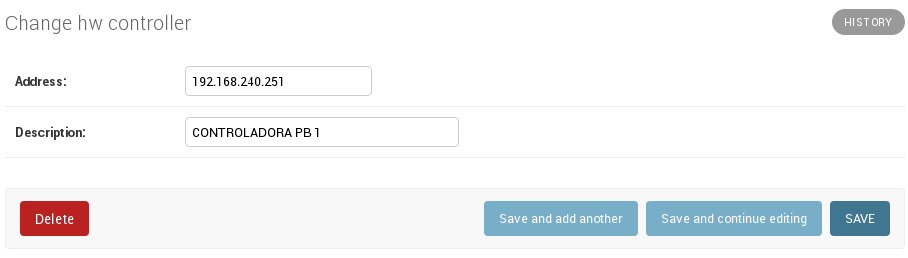
\includegraphics[width=1\textwidth]{/adm_hwcontroller.png}
\caption{Interfaz de administración de controladoras hardware}
\label{fig:adm_hwcontroller}
\end{figure}

\lstinputlisting[label = {retval:schema_main_hwcontroller}, caption = {Esquema de la tabla main\_hwcontroller, modelo HwController }, style = customconsole]{code/schema.main_hwcontroller}


\item \textbf{Device} Con el esquema detallado en el Listado~\ref{retval:schema_main_device}, se representa al dispositivo hardware que detecta el movimiento de una persona o interacciona con otros dispositivos físicos para dar una respuesta a un evento. Este modelo tiene los atributos: \textit{controller} para asociar el dispositivo a una controladora, \textit{description} para permitir al usuario establecer una descripción del dispositivo, \textit{mode} para definir una etiqueta que indique el modo de funcionamiento del dispositivo (entrada o salida) y \textit{location} para permitir al usuario establecer una descripción de la localización del elemento dentro del recinto a supervisar (ver Figura~\ref{fig:adm_device}).

\begin{figure}[hp]
\centering
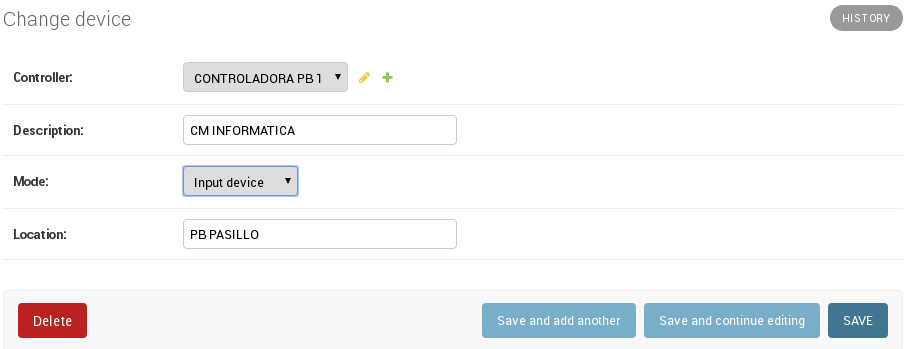
\includegraphics[width=1\textwidth]{/adm_device.png}
\caption{Interfaz de administración de dispositivos de entrada/salida}
\label{fig:adm_device}
\end{figure}

\lstinputlisting[label = {retval:schema_main_device}, caption = {Esquema de la tabla main\_device, modelo Device }, style = customconsole]{code/schema.main_hwcontroller}

\item \textbf{State} Con el esquema detallado en el Listado~\ref{retval:schema_main_state}, se representa un estado lógico de un dispositivo en un momento concreto y tiene los atributos: \textit{name} para permitir al usuario establecer un nombre del estado, \textit{description} para para albergar una descripción diferente al nombre si así se desea, \textit{image} para asociar una imagen o icono en concreto a ese estado, \textit{sound} para asociar un sonido en concreto a ese estado y \textit{color} para asociar un color específico sobre la información que se muestra  (ver Figura~\ref{fig:adm_state}).

\begin{figure}[hp]
\centering
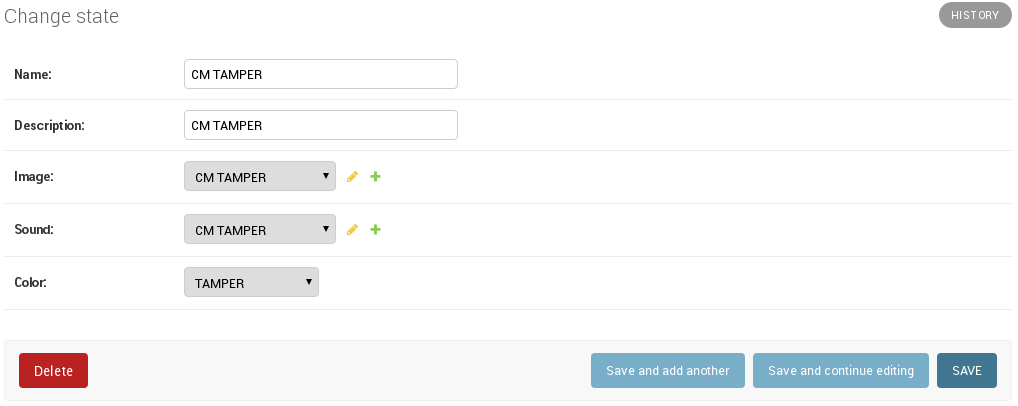
\includegraphics[width=1\textwidth]{/adm_state.png}
\caption{Interfaz de administración de los estados de un dispositivo}
\label{fig:adm_state}
\end{figure}

\lstinputlisting[label = {retval:schema_main_state}, caption = {Esquema de la tabla main\_state, modelo State }, style = customconsole]{code/schema.main_state}

\item \textbf{Image} Representa a una imagen que se asocia a un estado lógico de un dispositivo (ver Listado~\ref{retval:schema_main_image}) y tiene los atributos: \textit{description} para permitir al usuario establecer una descripción de la imagen o del estado que representa y \textit{url} para definir la ruta de la imagen dentro del servidor(ver Figura~\ref{fig:adm_image}). Una particularidad de este modelo es que además de poderse crear una instancia del mismo desde la interfaz de administración, también se puede crear una instancia de forma automática a través del modelo \textbf{ImageUploader} que está pensado solo para existir de forma temporal mientras el usuario sube una imagen personalizada a la aplicación (ver Figura~\ref{fig:adm_imageuploader}).

\begin{figure}[h]
\centering
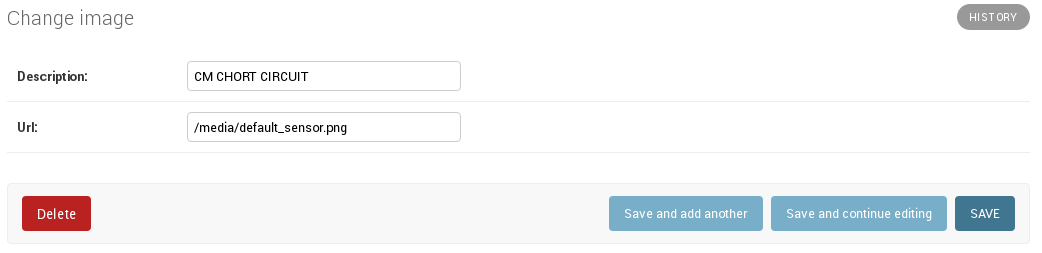
\includegraphics[width=1\textwidth]{/adm_image.png}
\caption{Interfaz de administración de la imagen asociada a un estado lógico}
\label{fig:adm_image}
\end{figure}

\lstinputlisting[label = {retval:schema_main_image}, caption = {Esquema de la tabla main\_image, modelo Image}, style = customconsole]{code/schema.main_image}

\begin{figure}[h]
\centering
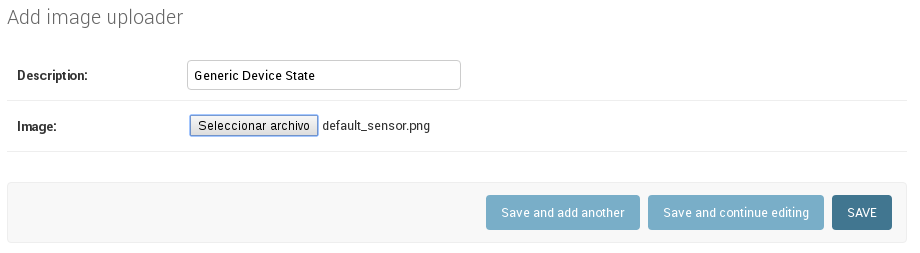
\includegraphics[width=1\textwidth]{/adm_imageuploader.png}
\caption{Interfaz de administración para la adición de imágenes personalizadas}
\label{fig:adm_imageuploader}
\end{figure}


\item \textbf{Event} Con el esquema detallado en el Listado~\ref{retval:schema_main_event}, se representa el evento generado por los diferentes cambios de estados físicos en un detector cualquiera en un momento dado. Estos cambios son reportados a la aplicación y tienen tiene los atributos: \textit{timestamp} para almacenar la hora y fecha en que se genera el evento y así poder disponer de una  traza temporal de los mismos, \textit{kind} para reflejar el tipo de evento según su origen, \textit{description} para mostrar la descripción del dispositivo que genera el evento, \textit{location} par indicar la localización del dispositivo que genera el evento y \textit{status} para indicar no solo el estado físico que representa el evento, sino también para diferenciar el evento visualmente de otros con un \textit{status} diferente (ver Figura~\ref{fig:adm_event}). 

\lstinputlisting[label = {retval:schema_main_event}, caption = {Esquema de la tabla main\_event, modelo Event }, style = customconsole]{code/schema.main_event}

\begin{figure}[h]
\centering
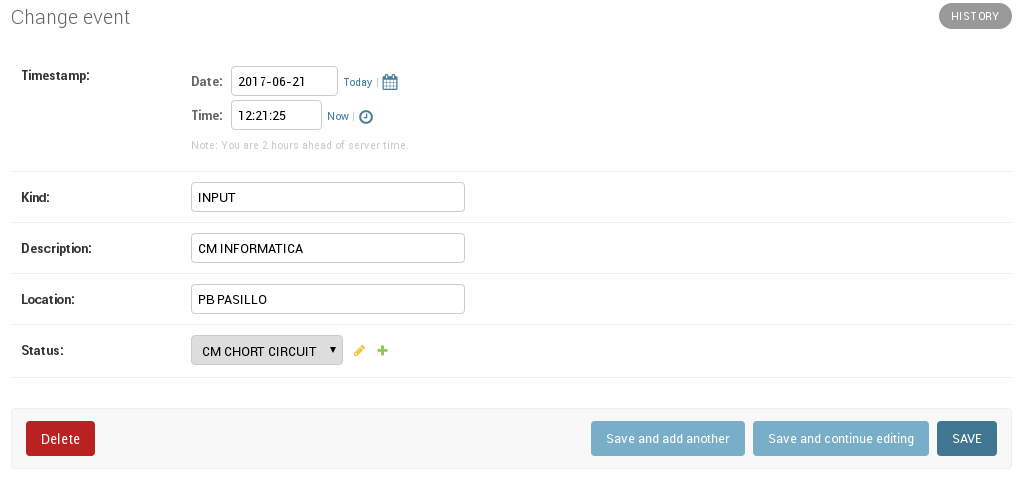
\includegraphics[width=1\textwidth]{/adm_event.png}
\caption{Interfaz de administración de controladoras hardware}
\label{fig:adm_event}
\end{figure}

\end{itemize}

Aunque ya disponemos de una interfaz de administración y de los modelos mínimos necesarios para representar la información generada por los detectores, puede resultar tedioso y repetitivo siempre que se elimine la \acs{BBDD} o su contenido, volver a crear manualmente a través de los formularios un mínimo de información útil para la explotación de la aplicación. Es muy común en otras aplicaciones tener a disposición del usuario; librerías y datos falsos que permitan en los primeros usos de la herramienta, hacerse una idea de cómo se representa la información en la misma. 

Teniendo en cuenta la idea anterior hemos optado por utilizar un método de aprovisionamiento de datos que ya nos provee el \textit{framework} de desarrollo de aplicaciones web \textit{Django}. Para ello hemos creado un \textit{Makefile}\footnote{\url{https://en.wikipedia.org/wiki/Makefile}} que nos facilite la ejecución de los comandos necesarios (ver Listado~\ref{code:makefile_django_loaddata}).

La plantilla desde la que se importan los datos (ver Listado~\ref{code:init_status_data_json}), es un fichero \acs{JSON} que contiene una lista de diccionarios con la información relevante y necesaria como pueden ser el modelo y los atributos de los datos que se quieren importar. 

Una vez que la importación se ha realizado satisfactoriamente podemos disponer de una información de carácter básico pero que nos da una idea de cómo se representan los diferentes eventos en el sistema(ver Figura~\ref{fig:init_data}).

\begin{figure}[h]
\centering
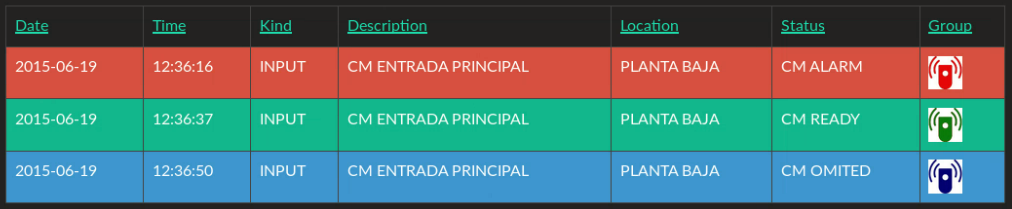
\includegraphics[width=1\textwidth]{/init_data.png}
\caption{Eventos generados tras el aprovisionamiento de la \acs{BBDD} de nuestra aplicación}
\label{fig:init_data}
\end{figure}

\lstinputlisting[label = {code:makefile_django_loaddata}, caption = {Comando de aprovisionamiento de la \acs{BBDD} \textit{SQLite} en \textit{Django}}, style = customconsole]{code/makefile.django_loaddata}

\hfill \linebreak

\lstinputlisting[label = {code:init_status_data_json}, caption = {Ejemplo de plantilla de aprovisionamiento de la \acs{BBDD} \textit{SQLite} en \textit{Django}}, style = customconsole]{code/init_status_data_json}

\subsection{Visualización de eventos}

La visualización de eventos a través de una interfaz que permita filtrarlos rápidamente y distinguirlos por el icono o color asociado al evento, puede resultar de gran utilidad para un sistema de seguridad. De hecho, la herramienta más básica en utilidad y funcionalidad es un log de eventos y lo que nos hemos planteado en esta iteración es ampliar este concepto para ofrecer una mayor usabilidad al usuario. Para esto además de mostrar un formato condicional según el estado lógico representado, también se ha añadido en la vista una barra de búsqueda que permite mostrar de forma dinámica aquellos eventos en los que coinciden los campos de: fecha, hora, descripción, localización y estado, con el parámetro introducido. Además los títulos de cada columna permiten ordenar los valores de la columna en cuestión, de manera ascendente o descendente según se desee (ver Figura~\ref{fig:basic_event_log}).

\begin{figure}[h]
\centering
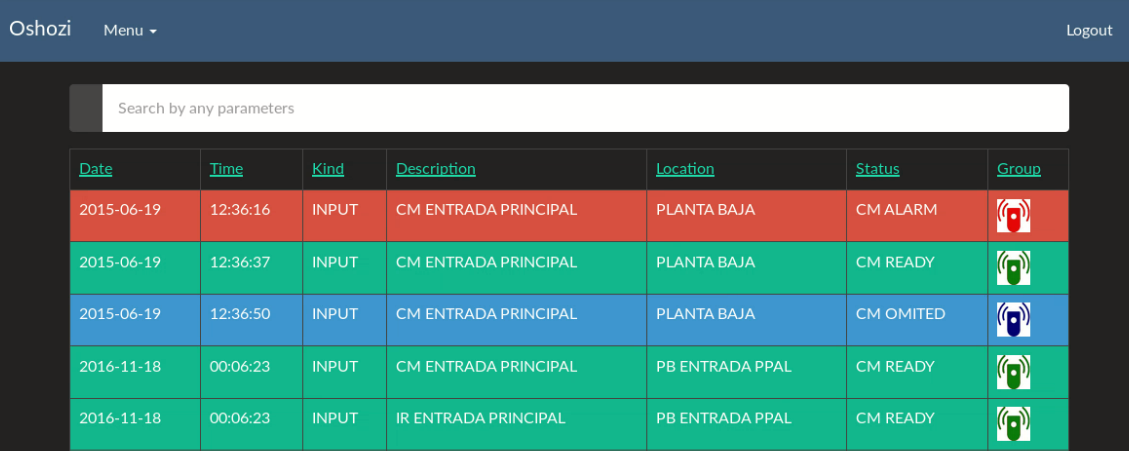
\includegraphics[width=1\textwidth]{/basic_event_log.png}
\caption{Visualización de eventos en Oshozi}
\label{fig:basic_event_log}
\end{figure}


\section{Iteración 4}

Con un método de emulación de los dispositivos hardware de seguridad y una aplicación con la capacidad de representar la información generada desde los detectores y las controladoras, nos queda pendiente desarrollar el nexo entre ambas partes de sistema (ver Figura~\ref{fig:incomplete_architecture}).

Por este motivo, en esta iteración se detalla cómo queda el sistema tras la creación de una \acs{API}-\acs{REST} que conecte ambas partes ya desarrolladas y las posibilidades que ofrece.

\begin{figure}[!h]
\centering
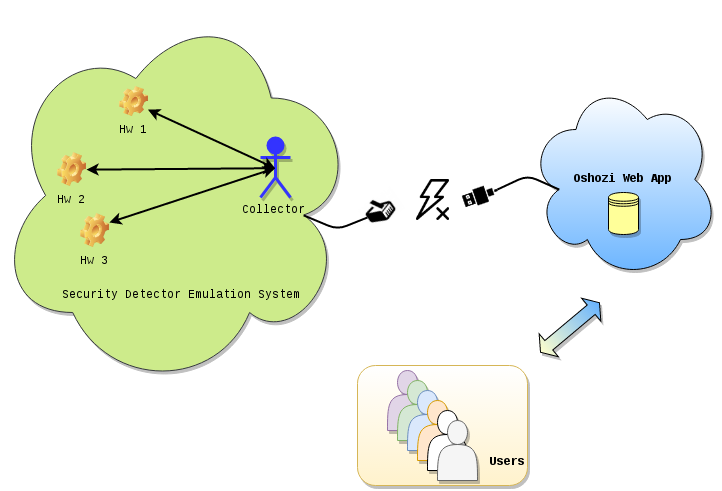
\includegraphics[width=1\textwidth]{/incomplete_arch.png}
\caption{Esquema de arquitectura incompleta}
\label{fig:incomplete_architecture}
\end{figure}

\subsection{\acs{API}-\acs{REST}}

Para la creación de nuestra \acs{API}-\acs{REST} lo primero que necesitamos es instalar los paquetes necesarios que ayudan a su creación y los complementarios que mejoran su uso (ver Listado~\ref{code:django.restframework_install}). Una ves hecho esto es necesario habilitar sus funcionalidades en nuestra aplicación a través del fichero \textit{settings.py} (ver Listado~\ref{code:django.restframework_enable}) y definir los \textit{endpoints} que se utilizarán para la gestión de la información entre el sistema de emulación y la aplicación web.

\lstinputlisting[label = {code:django.restframework_install}, caption = {Instalación \textit{Django} \acs{REST} \textit{Framework}}, style = customconsole]{code/django.restframework_install}

\lstinputlisting[label = {code:django.restframework_enable}, caption = {Habilitando \textit{Django} \acs{REST} \textit{Framework} en el fichero \textit{settings.py}},style=customhttp]{code/django.restframework_enable}

A continuación se explica para que se usa cada \textit{endpoint} y se muestra cuál es el aspecto visual de los mismos.

\begin{itemize}
\item \textbf{/api/} 

Por defecto cuando se consulta a través de un navegador web, se visualiza de forma navegable a través de un formulario, aunque también se permite la visualización en formato \acs{JSON} (ver Figura~\ref{fig:api_event_list}). Además admite consultas específicas aplicando filtros en la petición (ver Figura~\ref{fig:api_event_list_filter}).

\begin{figure}[!h]
\centering
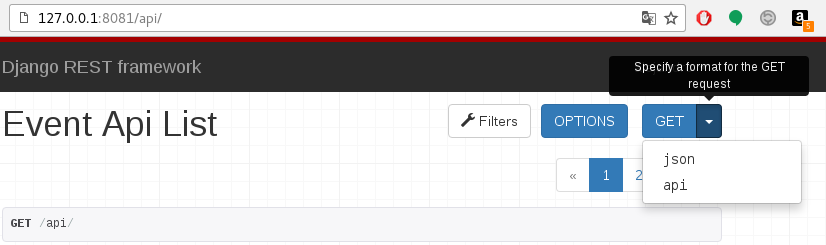
\includegraphics[width=1\textwidth]{/api_event_list.png}
\caption{Oshozi \acs{API}-\acs{REST}, listado de eventos del sistema}
\label{fig:api_event_list}
\end{figure}

Además de esto si pasamos un identificador de un evento existente en la \acs{BBDD} quedando el \textit{endpoint} construido como: \textbf{/api/id\_evento}, se nos retornan todos los campos de información almacenada sobre el evento (ver Figura~\ref{fig:api_event_getbyid}).

\begin{figure}[!h]
\centering
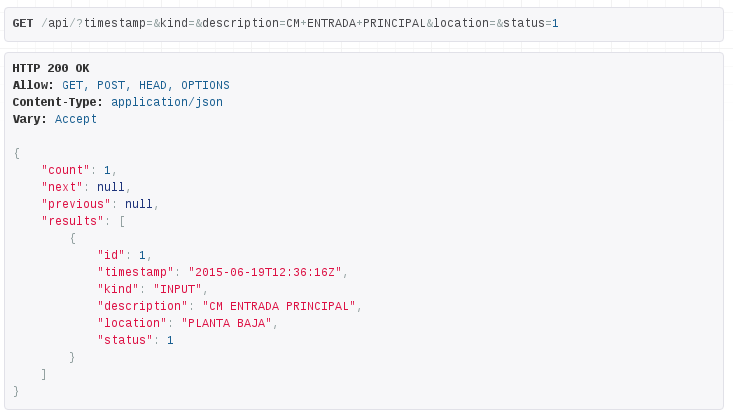
\includegraphics[width=1\textwidth]{/api_event_list_filter.png}
\caption{Oshozi \acs{API}-\acs{REST}, consulta de eventos del sistema filtrada}
\label{fig:api_event_list_filter}
\end{figure}

\begin{figure}[!h]
\centering
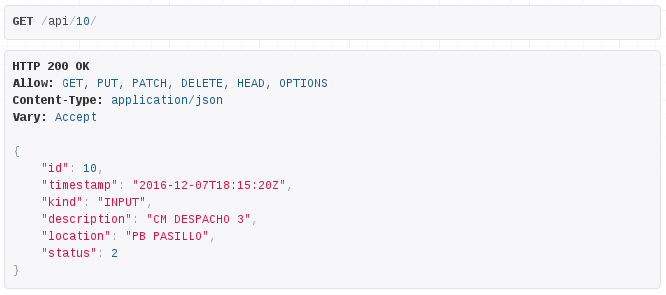
\includegraphics[width=1\textwidth]{/api_event_getbyid.png}
\caption{Oshozi \acs{API}-\acs{REST}, obtención de datos de un evento por id}
\label{fig:api_event_getbyid}
\end{figure}

Como no podía ser otra manera, nuestra \acs{API}-\acs{REST} también permite la creación de nuevos eventos en nuestra aplicación web a través de una operación \textit{POST}\footnote{Envía los datos a procesar a un recurso específico. \url{https://www.w3.org/Protocols/rfc2616/rfc2616-sec9.html}} (ver Listado~\ref{code:django.restframework_event_post}) sobre la url del \textit{endpoint} en cuestión (ver Figura~\ref{fig:api_event_post}).

\lstinputlisting[label = {code:django.restframework_event_post}, caption = {Oshozi \acs{API}-\acs{REST}, creación de un evento a través de línea de comandos},style=customconsole]{code/django.restframework_event_post}


\begin{figure}[!h]
\centering
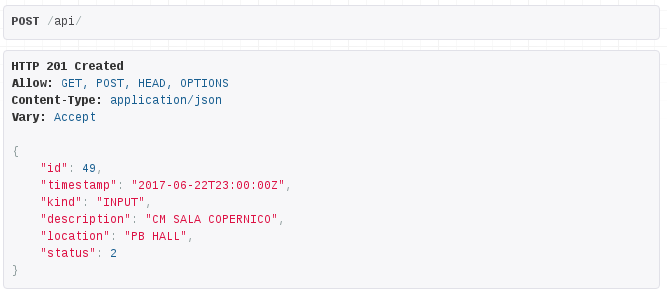
\includegraphics[width=1\textwidth]{/api_event_post.png}
\caption{Oshozi \acs{API}-\acs{REST}, evento creado a través de formulario}
\label{fig:api_event_post}
\end{figure}


\item \textbf{/api/hw/}

A través de este \textit{endpoint} podemos obtener un listado completo de todas las controladoras hardware dadas de altas en la aplicación, incluso a través de la línea de comandos de \textit{Python} (ver Listado~\ref{code:django.restframework_hw_list}). 

\lstinputlisting[label = {code:django.restframework_hw_list}, caption = {Oshozi \acs{API}-\acs{REST}, obtención de  listado de controladoras hardware a través de línea de comandos},style=customconsole]{code/django.restframework_hw_list}

De igual forma que en el caso de los eventos, si pasamos un identificador de una controladora hardware existente en la \acs{BBDD} quedando el \textit{endpoint} construido como: \textbf{/api/hw/id\_controladora}, se nos retornan todos los campos de información almacenada sobre la misma (ver Figura~\ref{fig:api_hw_getbyid}).

\begin{figure}[!h]
\centering
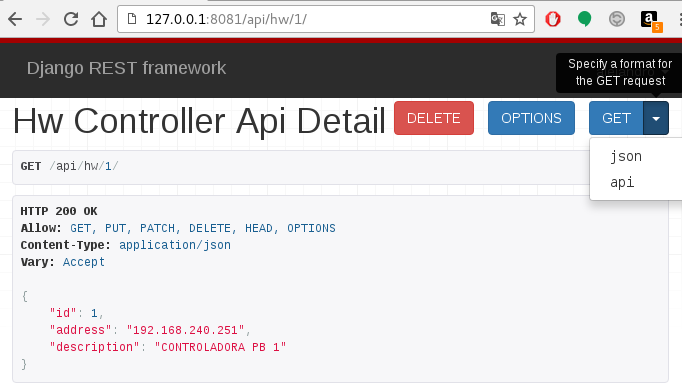
\includegraphics[width=1\textwidth]{/api_hw_getbyid.png}
\caption{Oshozi \acs{API}-\acs{REST}, obtención de datos de una controladora hardware por id}
\label{fig:api_hw_getbyid}
\end{figure}

\item \textbf{/api/device/}

Este \textit{endpoint} nos permite obtener un listado de todos los dispositivos (detectores, sensores y actuadores) que hay dados de alta en la aplicación. Al igual que en el caso de los \textit{endpoints} anteriores podemos obtener un listado con todos los dispositivos dados de alta, un dispositivo por su identificador (ver Figura~\ref{fig:api_device_getbyid}) y un dispositivo por una o varias de sus características o atributos (ver Figura~\ref{fig:api_device_filter}).

\begin{figure}[h]
\centering
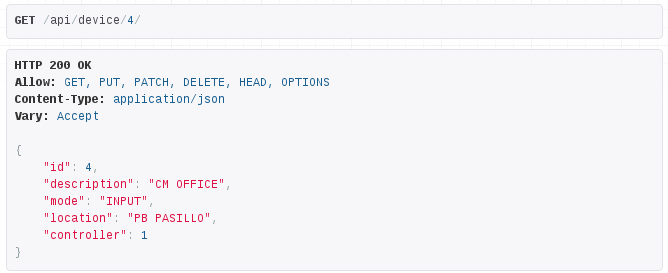
\includegraphics[width=1\textwidth]{/api_device_getbyid.png}
\caption{Oshozi \acs{API}-\acs{REST}, obtención de datos de un dispositivo hardware por id}
\label{fig:api_device_getbyid}
\end{figure}

\begin{figure}[!h]
\centering
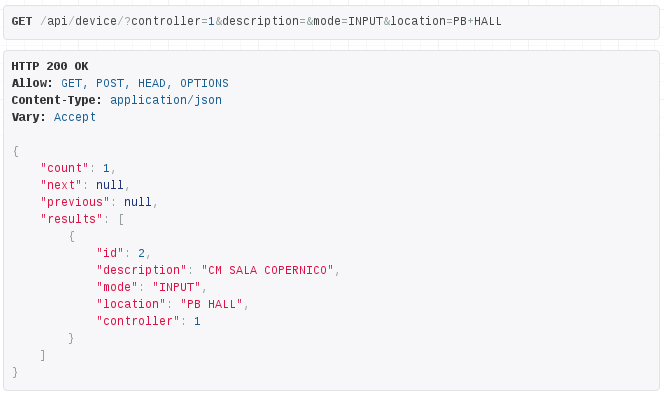
\includegraphics[width=1\textwidth]{/api_device_filter.png}
\caption{Oshozi \acs{API}-\acs{REST}, consulta de dispositivos del sistema filtrada}
\label{fig:api_device_filter}
\end{figure}

\end{itemize}

\subsection{Entorno de emulación}

Con la nueva \acs{API}-\acs{REST} desarrollada nos queda adaptar nuestro entorno de emulación para que pueda hacer uso de ella y así podamos completar la arquitectura de nuestro sistema (ver Figura~\ref{fig:complete_architecture}). 

\begin{figure}[!h]
\centering
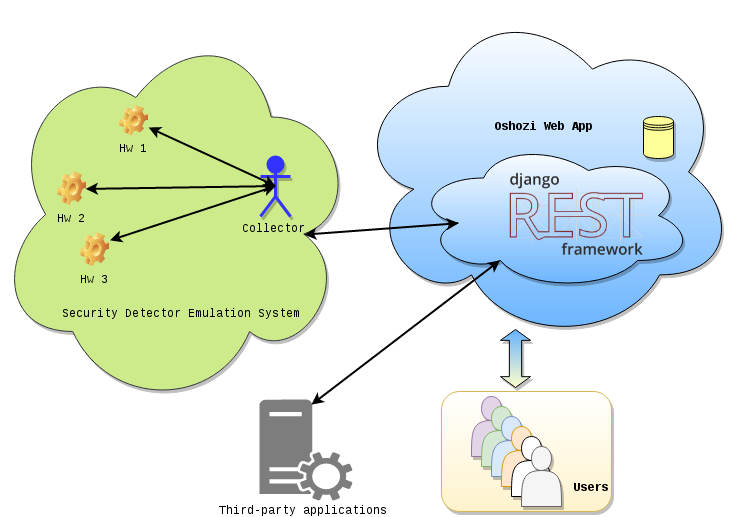
\includegraphics[width=1\textwidth]{/complete_arch.png}
\caption{Esquema de arquitectura completa}
\label{fig:complete_architecture}
\end{figure}

A continuación detallamos las funcionalidades que se han añadido al sistema de emulación hardware a través de los siguientes métodos (ver Figura:~\ref{fig:2_classes_collector}):

\begin{itemize}
\item \textbf{+ valid\_url(url: string): boolean} Comprueba si la url que se le pasa está disponible. Se utiliza para comprobar no solo que el servidor está arrancado sino también para comprobar la disponibilidad de cada uno de los \textit{endpoints} antes de hacer uso de ellos.

\item \textbf{+ get\_hw(address: string): dict} Este método sirve para obtener los datos de la controladora hardware, en caso que exista, desde la que se está recibiendo un evento. Para ello se hace una búsqueda aplicando como filtro la dirección ip que se le pasa al método y se recibe una lista que contiene los datos de la controladora coincidente. Se valida el contenido de la lista y se devuelve un diccionario que contiene los datos de la controladora en cuestión. De no encontrarse ninguna coincidencia se imprimen por pantalla varios mensajes que describen lo sucedido.

\item \textbf{+ get\_device(hw: dict): list} Permite obtener toda la lista de dispositivos que se encuentran dados de alta en el sistema y están asociados a una controladora hardware en concreto (la que se pasa al método). Para ello se hace una búsqueda aplicando como filtro el identificador de la controladora y se recibe una lista de todos los dispositivos coincidentes. De no encontrarse ninguna coincidencia se imprime por pantalla un mensaje que describe lo ocurrido.


\item \textbf{+ post\_event(event: dict): void} Este método no tiene ningún valor de torno y su única función es realizar la operación de inserción de un evento en la \acs{BBDD} a través de la \acs{API}-\acs{REST} de la aplicación.

\item \textbf{+ build\_event(node\_event: int, hw: dict, device\_list: list): boolean} Este método es el encargado de construir el evento que se está generando a través de la plantilla de emulación de estados físicos, procesada por el sistema de emulación. Para ello se evalúan los datos que se le pasan al método, donde:

\begin{itemize}
  \item \textbf{node\_event} es un entero que indica la posición que ocupa el detector, que está generando un estado el evento, en la controladora hardware que lo supervisa.

  \item \textbf{hw} es un diccionario con los datos de la controladora hardware que supervisa al detector que está generando el evento.

  \item \textbf{device\_list} es una lista que contiene los datos de todos los dispositivos asociados a la controladora hardware que supervisa al detector que está generado el evento.
  \end{itemize}

Teniendo en cuenta los datos anteriores y entrelazando la información (ver Listado~\ref{code:server.build_event}) es posible generar un nuevo evento, que en caso de considerarse nuevo, será notificado a nuestra aplicación web.

\hfill
\lstinputlisting[label = {code:server.build_event}, caption = {Método \textbf{buid\_event}, entorno de emulación}, style=customhttp]{code/server.build_event}

\item \textbf{+ new\_event(event: dict, device: dict): boolean}  Este método comprueba si el \textbf{status} del último evento generado por el dispositivo que se le pasa es igual al \textbf{status} del evento que se le pasa. Con esta comprobación lo que se pretende es evitar la inserción de eventos en la \acs{BBDD} que ya se han registrado en la aplicación y que no aportan un valor informativo añadido. 

\end{itemize}

\begin{figure}[h]
\centering
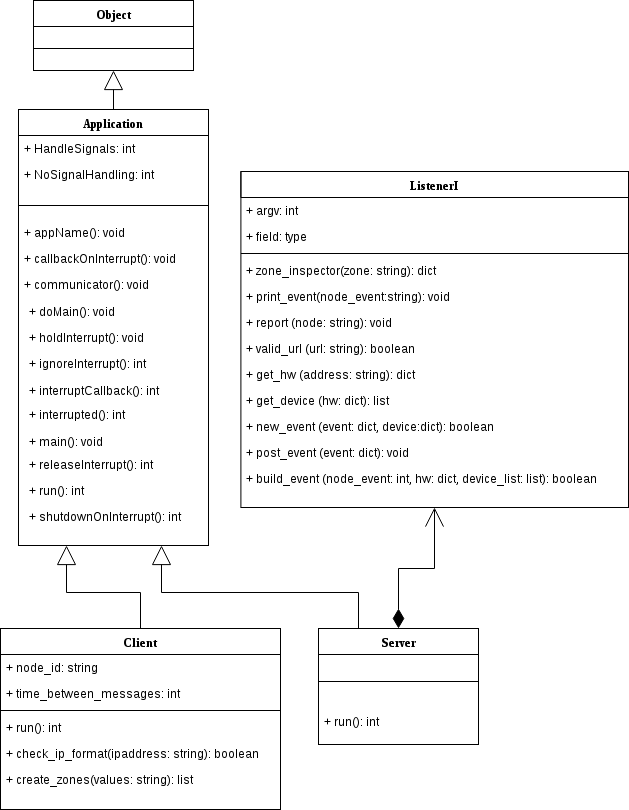
\includegraphics[width=0.8\textwidth]{/2_classes_collector.png}
\caption{Diagrama de clases del entorno de emulación}
\label{fig:2_classes_collector}
\end{figure}

\section{Iteración 5}
Como no podía ser de otra forma, un sistema de seguridad no solo tiene que ser útil por sus prestaciones, también debe de disponer de unos mecanismos mínimos que lo hagan seguro. Hasta el momento no habíamos podido invertir tiempo en restringir el uso de la aplicación o su \acs{API}-\acs{REST} porque no contábamos con una arquitectura terminada que abarcase desde el detector hasta la aplicación de gestión. Por este motivo en esta iteración me he centrado en la implantación de un sistema de autenticación  y en la mejora de algunos aspectos visuales de la aplicación.

\subsection{Autenticación}

Como muchos \textbf{frameworks} de desarrollo que gozan de una amplia comunidad de usuarios y desarrolladores, \textit{Django} nos facilita diversos medios y herramientas que nos permiten crear sistemas de autenticación a través de varios mecanismos más o menos complejos, según las necesidades y preferencias del desarrollador.

Para elegir el mecanismo de autenticación adecuado a nuestra aplicación, se han tenido en cuenta las siguientes premisas:

\begin{itemize} 
\item Nuestra aplicación va orientada a instalaciones de \acs{GII} y \acs{GIII}.
\item Mayoritariamente en el resto de los sistemas comerciales que cubren este nicho, se emplea como mecanismo básico de seguridad de la herramienta el uso de un \textbf{usuario} y \textbf{contraseña}.
\item Aunque no es el aspecto más importante, se ha tenido en cuenta la dificultad de implementación he implantación del mecanismo.
\end{itemize}
 
Teniendo en cuenta las razones anteriormente expuestas, he optado por permitir el uso de las funcionalidades de la aplicación únicamente a aquellos usuarios que previamente hayan iniciado sesión en la misma. 

Para ello se ha creado una interfaz de \textit{login} (ver Figura~\ref{fig:django_login_view}) que se muestra por defecto siempre que el usuario no está autenticado he intenta acceder a cualquiera de las interfaces restantes de la aplicación.

Esto se ha conseguido habilitando la herramienta de autenticación en el fichero \textit{settings.py} (ver Listado~\ref{code:django.basic_auth}) y añadiendo restricciones en las vistas (\textit{views}, tienen el rol de controlador según el patrón \acs{MVC}) (ver Listado~\ref{code:django.views_auth}).

\begin{figure}[h]
\centering
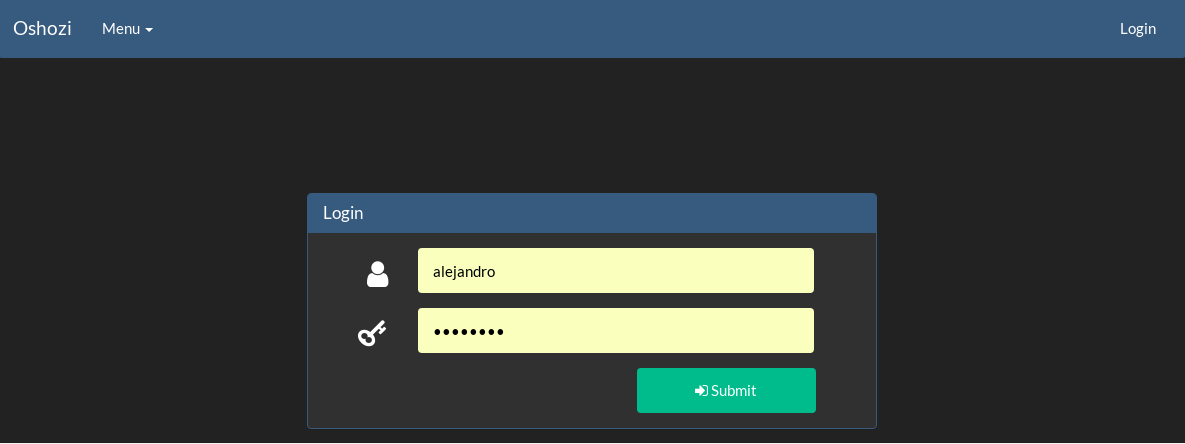
\includegraphics[width=1\textwidth]{/django_login_view.png}
\caption{Interfaz de autenticación de Oshozi}
\label{fig:django_login_view}
\end{figure}

\lstinputlisting[label = {code:django.basic_auth}, caption = {Habilitando la herramienta de autenticación en el fichero \textit{settings.py}}, style=customhttp]{code/django.basic_auth}

\lstinputlisting[label = {code:django.views_auth}, caption = {Restricción de autenticación aplicada para la visualización de \textit{index.html}}, style=customhttp]{code/django.views_auth}

Además de esto, para mejorar la experiencia del usuario se definen varios mensajes que son pasados desde la vista \textbf{login\_view} hasta la plantilla (\textit{template}, tienen el rol de vista según el patrón \acs{MVC}) de \textit{login} cuando:

\begin{itemize}
\item El \textbf{usuario} o la \textbf{contraseña} introducidos son incorrectos (ver Figura~\ref{fig:django_wrong_auth}).
\item Los campos de \textbf{usuario} y \textbf{contraseña} se han dejado en blanco (ver Figura~\ref{fig:django_invalid_form}).
\end{itemize}

\begin{figure}[h]
\centering
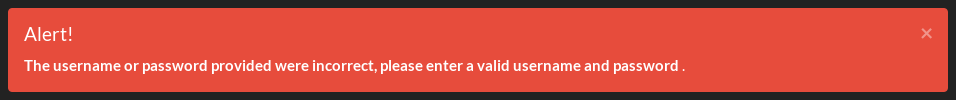
\includegraphics[width=1\textwidth]{/django_wrong_auth.png}
\caption{Mensaje de error que se lanza cuando el usuario o la contraseña son inválidos}
\label{fig:django_wrong_auth}
\end{figure}

\begin{figure}[h]
\centering
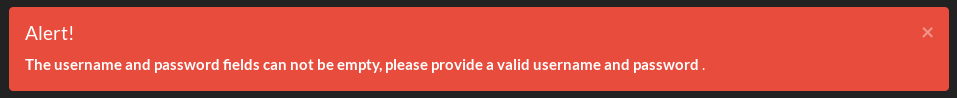
\includegraphics[width=1\textwidth]{/django_invalid_form.png}
\caption{Mensaje de error que se lanza cuando el formulario de \textit{login} se dejan en blanco}
\label{fig:django_invalid_form}
\end{figure}

Conseguido el mecanismo de autenticación de nuestra aplicación nos queda pendiente la implantación de un nivel similar de seguridad en la \acs{API}-\acs{REST} para evitar usos desautorizados de la misma. Para ello \textit{Django} \acs{REST} \textit{Framework} también nos propone varios mecanismos y herramientas, aunque hay una librería que destaca por su simplicidad y facilidad de uso: \textbf{django-rest-auth}.

Para usar esta librería primero necesitamos instalarla (ver Listado~\ref{code:django.rest_auth}) y habilitar su uso en nuestra aplicación como hemos venido haciendo con el resto de librerías hasta el momento (ver Listado~\ref{code:django.rest_auth_enable}).

\hfill
\lstinputlisting[label = {code:django.rest_auth}, caption = {Instalación de la librería \textbf{django-rest-auth}}, style=customconsole]{code/django.rest_auth}

Una vez habilitada la librería en nuestra aplicación debemos, parametrizar en la misma quién tiene permisos para usar nuestra \acs{API}-\acs{REST}, los usuarios autenticados o únicamente los usuarios administradores. En nuestro caso he decido que solo se va a permitir el uso a los usuarios administradores debido a la criticidad de la información manejada (ver Listado~\ref{code:django.restframework_config}).

\lstinputlisting[label = {code:django.rest_auth_enable}, caption = {Habilitando \textbf{django-rest-auth} en el fichero \textit{settings.py}}, style=customhttp]{code/django.rest_auth_enable}

\lstinputlisting[label = {code:django.restframework_config}, caption = {Parámetros de configuración de \textit{Django} \textit{\acs{REST}} \textit{Framework}}, style=customhttp]{code/django.restframework_config}

Llegados a este punto comprobamos satisfactoriamente que sólo un usuario administrador puede hacer uso de las funcionalidades de la \acs{API}-\acs{REST} (ver Figura~\ref{fig:django_apirest_nonloged} y Figura~\ref{fig:django_apirest_loged}).

\begin{figure}[!h]
\centering
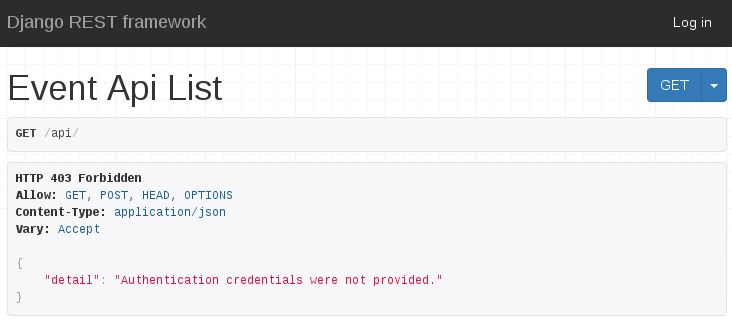
\includegraphics[width=1\textwidth]{/django_apirest_nonloged.png}
\caption{Apariencia de la \acs{API}-\acs{REST} sin usuario administrador autenticado}
\label{fig:django_apirest_nonloged}
\end{figure}

\begin{figure}[!h]
\centering
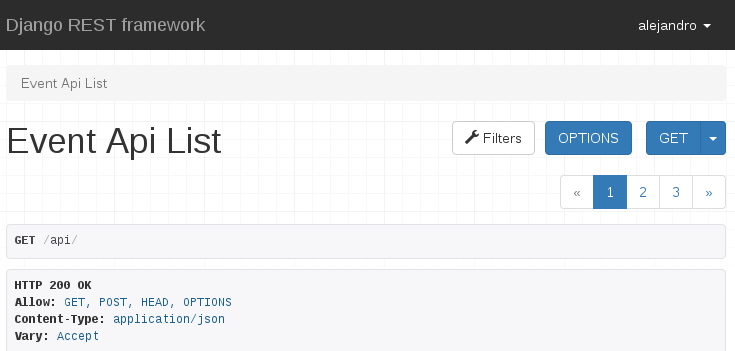
\includegraphics[width=1\textwidth]{/django_apirest_loged.png}
\caption{Apariencia de la \acs{API}-\acs{REST} con usuario administrador autenticado}
\label{fig:django_apirest_loged}
\end{figure}

\subsection{Mejoras en la experiencia del usuario}

Unos de los aspectos más importantes a tener en cuenta cuando se desarrolla una aplicación web son; la experiencia del usuario y la usabilidad. Características que en los sistemas tradicionales de seguridad quedan relegados a un plano totalmente secundario y en algunos sistemas prácticamente inexistentes. 

Por este motivo en esta iteración intentamos corregir esa tendencia y hacemos uso de la herramienta \textit{Font Awsome} para añadir iconos a través de una combinación de caracteres sin la necesidad de utilizar imágenes (ver Figura~\ref{fig:django_fontawsome_icon}). Para ello solo es necesario añadir la referencia al archivo \textit{font\_awsome.min.css} en la cabecera de nuestra plantilla web (ver Listado~\ref{code:django.fontawsome}).

\begin{figure}[!h]
\centering
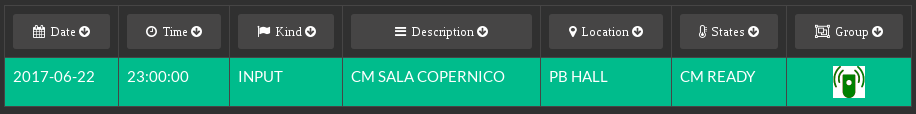
\includegraphics[width=1\textwidth]{/django_fontawsome_icon.png}
\caption{Uso de \textit{Font Awsome} en Oshozi}
\label{fig:django_fontawsome_icon}
\end{figure}

\lstinputlisting[label = {code:django.fontawsome}, caption = {Habilitando \textit{Font Awsome} en la cabecera de la plantilla \textit{base.html}}, style=customhttp]{code/django.fontawsome}

Además de esto se ha añadido un botón de refresco (ver Figura\ref{fig:django_refresh_btn}) que llama a una función \textit{javascript} (ver Listado\ref{code:django.btn_angularjs}), para que la platilla muestre por pantalla únicamente aquellos eventos que no se han recibido después de la carga de los datos en la interfaz y que no se están visualizando, sin necesidad de recargar toda la página web. Esto se consigue gracias a \textit{AngularJS}, que por su concepción, cuando se hace una petición de una página web si ya dispone de datos de la misma, sólo se trae del servidor aquellos datos que son nuevos o han sido modificados.

\begin{figure}[!h]
\centering
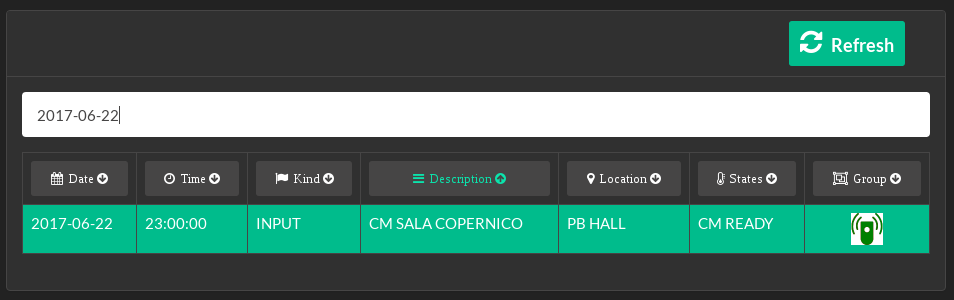
\includegraphics[width=1\textwidth]{/django_refresh_btn.png}
\caption{Botón de refresco de eventos en Oshozi}
\label{fig:django_refresh_btn}
\end{figure}

\lstinputlisting[label = {code:django.btn_angularjs}, caption = {Función \textit{javascript} ytilizada para el refresco de eventos}, style=customhttp]{code/django.btn_angularjs}
